\section{PROPOSED FRAMEWORK}
\label{sec:framework}
\begin{figure}
    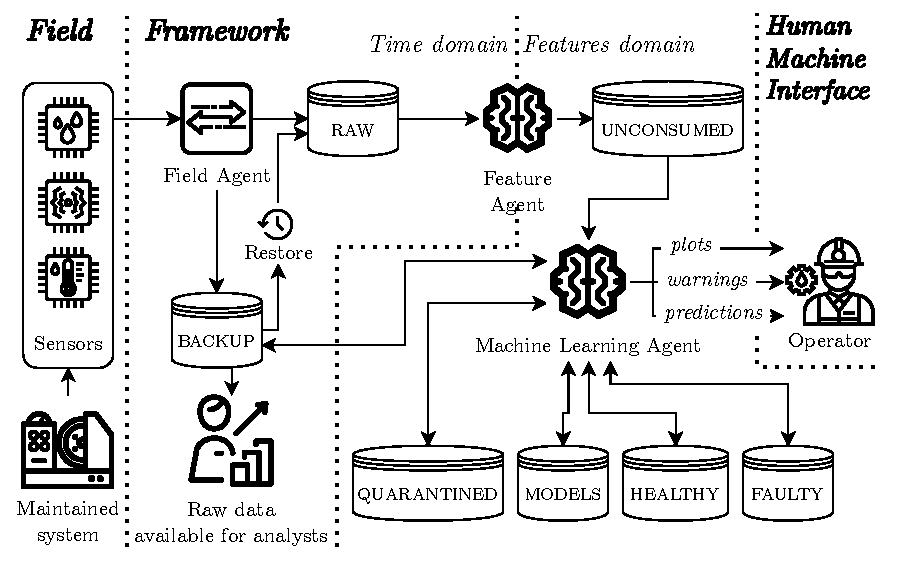
\includegraphics[width=\linewidth]{images/Framework_structure.pdf}
    \caption{The structure of the proposed framework}
    \label{fig:framework_structure}
\end{figure}

The solution developed in this project is thought to be set up on a new device, and linked to the sensors of the most informative quantities of the system.
In the first phase of commissioning, the framework collects the data, extracts the features and stores them. When the data collected is enough to characterize all the modes of operation of the maintained system, the UML model can be trained. Finally, the framework continues collecting new data, extracting the features, and evaluating the new data. The framework now produces a Novelty Metric (NM) that quantifies the novelty of new data. 
This phase can last indefinitely, when the NM overshoots a certain threshold, a warning is issued to the maintenance team. They can then decide to perform a maintenance action or to continue monitoring the system. If they declare the system as healthy, the framework can be retrained with the new data, to update the UML model. Otherwise, a second UML model can be trained to characterize the newly discovered fault and perform FD in the future.

\subsection{software agent}
The proposed framework is based on software agents. Each agent is autonomous and performs a specific task. The developed agents, as shown in Fig. \ref{fig:framework_structure}, are:
\begin{itemize}
    \item \textbf{Field Agent (FiA)}: responsible for the synchronous sampling of the data.
    \item \textbf{Feature Agent (FA)}: extracts the features from the time series.
    \item \textbf{Machine Learning Agent (MLA)}: trains the UML algorithms and then performs ND, FD and PM. It reports the results to the user.
\end{itemize}

\subsection{Database}
All the Agents are connected to a common database. In the case of the PC implementation, MongoDB has been used. In the case of the Edge implementation, the data are stored directly in the microcontroller's memory.
Regarding the structure shown in Fig. \ref{fig:framework_structure}, the MongoDB database is composed of seven collections: \emph{Raw} containing the time series, \emph{Unconsumed} containing the features to be evaluated by the MLA, \emph{Quarantined, Healthy and Faulty} containing the features that have been flagged as novelty, normal or faulty, respectively, and \emph{Models} containing the UML models. The collection \emph{Backup} is general purpose.

\subsection{Multiple Instances}
As shown in Fig. \ref{fig:multiple_instances}, the framework can be implemented in multiple instances. This is useful to better isolate the location of the anomaly in a complex system. The larger the sensors that a single instance of the framework is connected to, the more difficult it is to isolate the anomaly.

\begin{figure}
    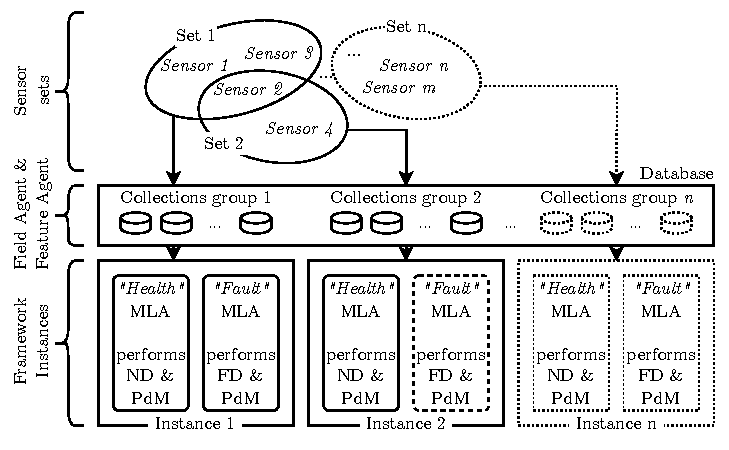
\includegraphics[width=\linewidth]{images/FrameworkInstances.pdf}
    \caption{Multiple instances implementation of the framework}
    \label{fig:multiple_instances}
\end{figure}